\documentclass{eage19}

\graphicspath{{images/}}
\begin{document}

\section{Introduction}
Water-coning has been observed in those oil producing wells in which water encroaches from below and shuts-off some or most of the oil production \citep{Muskat1934}. This problem typically occurs when a critical production rate ($q_{cr}$) is exceeded. The definition of such critical production rate is complicated, and this makes operation of oil wells near bottom aquifers complex. In general, one would like to operate at a maximum production rate ($q$) while ensuring that $q<q_{cr}$. Due to uncertainty in the value of $q_{cr}$ for a given well, dynamics of watercone development should be captured.

Most current solutions are \textit{reactive} rather than \textit{proactive}. In other words, after a watercone has encroached into an oil producer, an \textit{ad-hoc} remedy is considered. The solution can be a reduction of the production flow rate \citep{Larry2007}, the use of chemicals such as foams \citep{Persoff1990} and gels \citep{Seright1993}, or even the use of dual-completion technology \citep{Ould2004}. As soon as water-cone interferes with an oil producer, it will disconnect part of its oil flow network. Therefore, oil production does not recover to the level prior to watercone encroachment, even when the \textit{reactive} treatment is successful.

Existing methods of estimating water-coning are based on the correlations built from reservoir simulations \citep{Kuo1983} or on the analytic solutions using simplified assumptions \citep{Bournazel1971,Egbe2005}. In this paper, we present a multi-physics approach to estimating encroachment of a watercone. The watercone development is captured using a commercial reservoir simulator, while the electromagnetic response to the watercone is captured using electromagnetic simulations. Our approach is then used in to design and optimize the near-wellbore electromagnetic sensing tools in uncased wells and for wells cased with resistive fiberglass casing.

\section{Method and Theory}

In this paper we consider a homogeneous oil reservoir underlain by an aquifer. The distance between the wellbottom and the aquifer is 40 m. The porosity of the rock is $\phi =20$\%, the horizontal permeability is $k_h =100$ mD, and the ratio of vertical to horizontal permeability is $k_v/k_h=0.33$. The water saturations in the oil reservoir and the aquifer are $S_w =0.2$ and 0.8, respectively. The top of the reservoir is at a depth of 2600 m, and the production rate is 200 bpd. The reservoir brine salinity is 200000 ppm, typical of the Middle Eastern reservoir brines \citep{Staff1959}.

We discuss two approaches for calculating shape of the water front. In the first case, we evenly grow a geometric cone whose height is equal to its radius. In the  second case, the dynamics of water-cone growth is captured with the CMG reservoir simulator. The saturation distribution at various stages of watercone growth is used as an input to the electromagnetic (EM) simulations, where we used the AC/DC module of COMSOL. This way, we can understand the dynamic EM response of the watercone growth for different tool parameters. Note that we use the reservoir simulator only to verify the proposed technology. Analytical solutions, field data, or other input data can be used instead.

The formation resistivity is described by the classic Archie's law \citep{ARCHIE1942},

\begin{equation}
S_{w} = \left( \frac{a}{\phi^m}\frac{R_w}{R_t}\right)^{\frac{1}{n}},
\label{archies}
\end{equation}

where $R_w$ and $R_t$ are the water and saturated formation resistivities, $a$ is the tortuosity exponent, $m$ is the cementation exponent and $n$ is the saturation exponent. The parameters in Eq. \ref{archies} are listed in Table \ref{geoelectric_table} for a carbonate and a sandstone formation.

\begin{table}[h!]
\begin{center}
\begin{tabular}{|c|c|c|c|c|c|}
\hline
\textbf{Rock} & \textbf{a} & \textbf{n}& \textbf{m} & \textbf{$R_t$ oil reservoir, $Ohm \cdot m$}& \textbf{$R_t$ aquifer, $Ohm \cdot m$}  \\
\hline
Carbonate    & 1 & 2 & 2 & 27.5 & 1.72  \\
Sandstone    & 0.62 & 2.15 & 2 & 18.74 & 1.17   \\
\hline
\end{tabular}
\caption{Archie's parameters and corresponding resistivities}
\label{geoelectric_table}
\end{center}
\end{table}

\begin{figure}[h!]
	\begin{minipage}{0.54\linewidth}
		\center{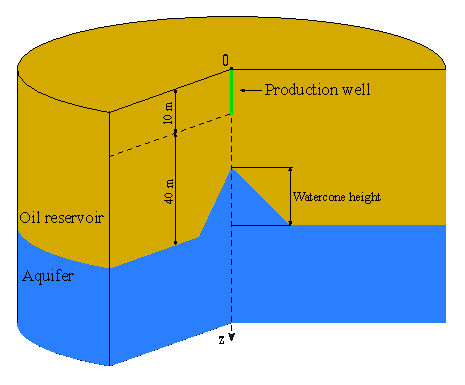
\includegraphics[clip,width=1\linewidth]{scheme_watercone.eps} \\ a)}
	\end{minipage}
	\hfill
	\begin{minipage}{0.42\linewidth}
		\center{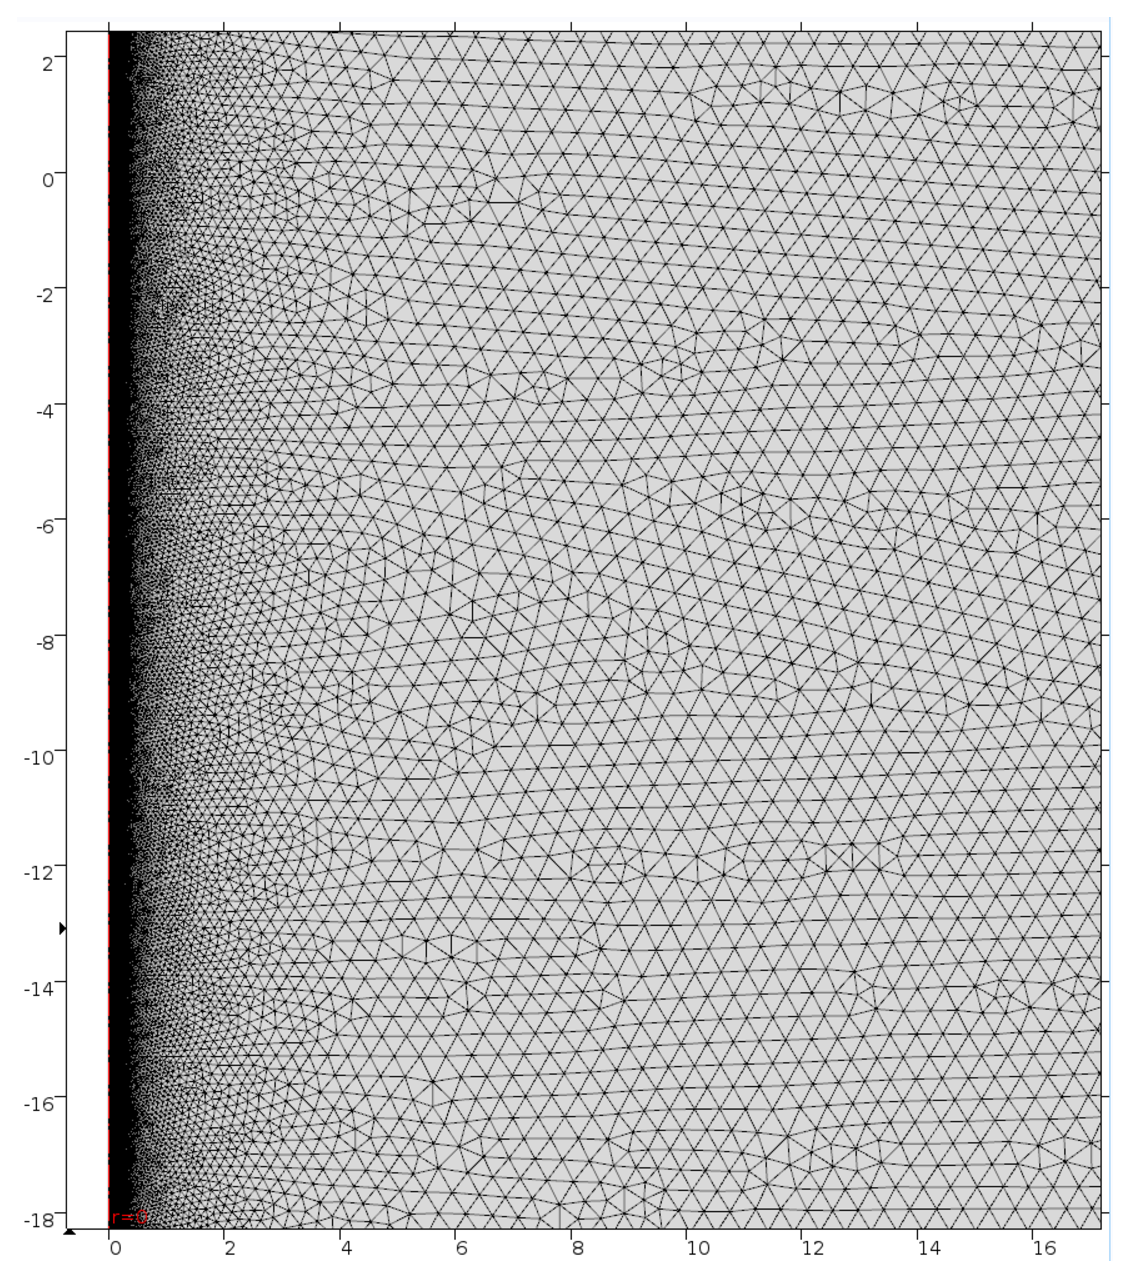
\includegraphics[clip,width=1\linewidth]{mesh.eps} \\ b)}
	\end{minipage}
	\caption{a)  Schematic representation of waterconing occurred in thick oil reservoir and b) part of the mesh used in the simulation}
	\label{scheme_wconning_mesh}\
\end{figure}

\section{Results}

To calculate the apparent  resistivity from induction signals, we use a homogeneous medium approximation. The measured signals are $\varphi$, the phase, and $A$, the attenuation  of the electromotive force induced in the receiving coil by magnetic field:

\begin{equation}
H_{z} = \frac{M_{z}}{2\pi L^3}e^{-kL}(1+kL), \hspace{0.5cm}
a = Re(H_{z}) , \hspace{0.5cm}
b = Im(H_{z})
\end{equation}

\begin{equation}
\varphi = \arctan \left( \frac{b}{a} \right), \hspace{0.5cm}
A = 20 \log_{10} \left( \frac{1}{2\pi L^3 \sqrt{a^2+b^2}} \right)
\label{varphi}
\end{equation}
Here $\omega$ = the circular frequency, $L$ = distance between transmitter and receiver;  k =  $\sqrt{- i \omega \mu /\rho}$; the rock is nonmagnetic with the magnetic permeability $\mu= 1$; and $\rho$ = electrical resistivity. EM source with the magnetic moment, $M_{z}$, of 10 $Am^2$ is located at the origin. To exclude direct field we use the three-coil tools: one transmitter and five pairs of receiving coils at 5.5 and 6; 6.4 and 7; 7.3 and 8; 8.2 and 9; and 9.1 and 10 meters. The most distant coil is located at the wellbottom. The EM signals are  transformed into apparent electrical resistivities for better visualisation.

First, a response from a uniformly growing water cone is modeled without taking into account the reservoir porosity and permeability. Height of the cone is equal to its base radius, see Fig.\ref{scheme_wconning_mesh} a. This idealization is far from the the CMG output, Fig~\ref{stages_figure} a, and we used it to identify the effect of watercone on the tool response. Fig.~\ref{scheme_wconning_mesh} b shows the part of mesh used in the simulation. The total mesh area is 20000 m$^2$, average element quality is 0.97 with the element sizes that vary from 0.002 to 0.5 m, depending on the region. Figure ~\ref{signals1} shows change in apparent resistivity during watercone development for the simplified model of the cone. The greater the distance between the coils, the greater the coverage area of the device. Longer tools are better in detecting decreases of electrical resistance of the rock. The dashed line in Fig.~\ref{signals1} depicts the measured signal that is greater by 3\% (typical measurement error) than the response from rock without watercone. At this stage, we can say that the electrical rock resistance is changing and cone growth is occurring.


\begin{figure}[h!]

		\centering
		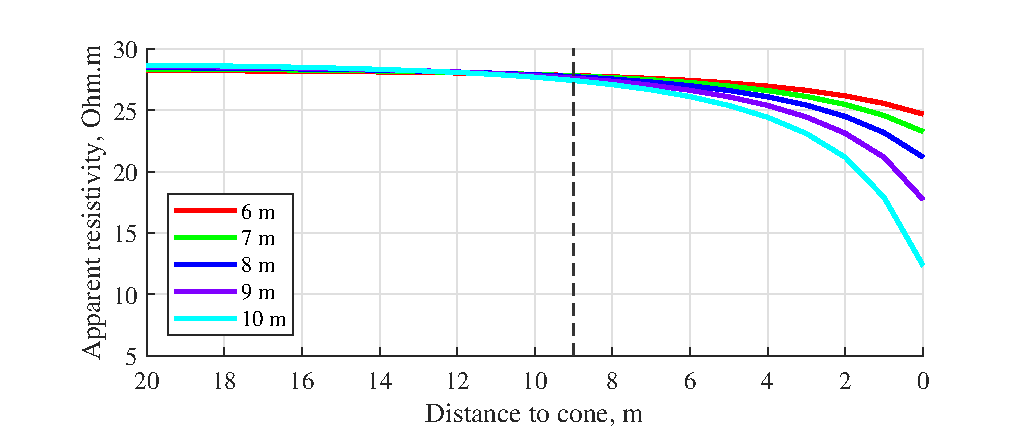
\includegraphics[clip,width=0.85\linewidth]{phase_diff.eps}

	\caption{Apparent resistivity calculated at frequency = 1 kHz vs. distance to cone. EM response is calculated from the simple cone model in Fig.~\ref{scheme_wconning_mesh} a. Five three-coil tools are considered. The dashed line shows the longest tool response that exceeds 3\%}
	\label{signals1}\
	
\end{figure}



  \begin{minipage}{\textwidth}
	\begin{minipage}[b]{0.52\textwidth}
		\centering
		\includegraphics[scale=0.25]{cone_stages2.eps}
%		\rule{6.4cm}{3.6cm}
		\captionof{figure}{Stages of water cone growth, CMG simulation results. Dashed lines shows location of water front at different times}
		\label{stages_figure}
	\end{minipage}
	\hfill
	\begin{minipage}[b]{0.44\textwidth}
		\centering


\begin{tabular}{lll}
\textbf{Stage \#} & \textbf{\begin{tabular}[c]{@{}l@{}}Time, \\ months\end{tabular}} & \textbf{\begin{tabular}[c]{@{}l@{}}Distance \\ to cone, m\end{tabular}} \\
0                 & 0                                                                & 40                                                                      \\
1                 & 17                                                               & 33.7                                                                    \\
2                 & 33                                                               & 26.2                                                                    \\
3                 & 49                                                               & 15.8                                                                    \\
4                 & 53                                                               & 11.2                                                                    \\
5                 & 55                                                               & 3.7                                                                     \\
6                 & 56                                                               & 0
\vspace{1.2cm}
\end{tabular}



				\captionof{table}{Stages and time of watercone growth, distance from wellbottom to the cone \\ \vspace{0.14cm}}	
				\label{stages_table}
%\vspace{0.1 cm}
\end{minipage}
\end{minipage}


Water-cone growth is now simulated using CMG, see  Fig.~\ref{stages_figure} and Table ~\ref{stages_table}. Figure ~\ref{signals2} shows change in the measured signal depending on the production stage. Here, the influence of the cone can be detected between the second and third stages of production. A more realistic shape of the cone allows us to detect it between 15 and 25 meters away from the well. One can observe that the significant change in signal is observed at stage 3 for the apparent resistivity. The relative change in apparent resistivity between  stages 1 and 2 is slightly more than 3\%, which is typical of the tool measurement error; signal change of more than 3\% can be measured. It is worth noting that the shape of the watercone obtained with the CMG simulator is different from the idealized cone. Comparing Figs. ~\ref{signals1} and ~\ref{signals2} one can see that shape of the water front has significant influence on the EM response and the cone can be detected farther away from the wellbottom. Therefore, in electromagnetic modeling of an oilfield development process, one should pay attention to reservoir simulation and use more realistic models of fluid distributions around wellbore.

\begin{figure}[h!]
	\centering
	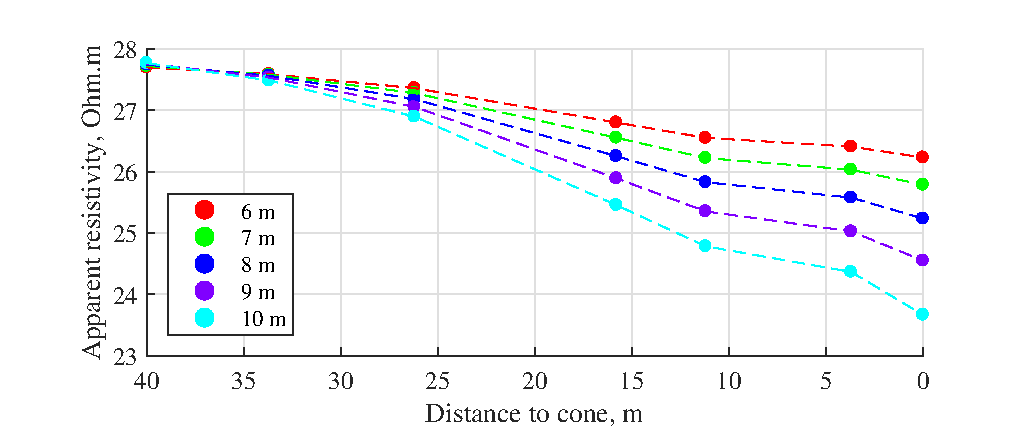
\includegraphics[clip,width=0.85\linewidth]{phase_diff_cmg.eps}
	\caption{Apparent resistivity at frequency = 1 kHz vs. distance to the cone, Table~\ref{stages_table}. Dynamic saturation distribution is obtained using reservoir simulation, Fig.~\ref{stages_figure}. Five three-coil tools are considered}
	\label{signals2}
\end{figure}

\section{Conclusions}

We have conducted reservoir simulations followed by electromagnetic (EM) simulations that use the computed fluid distributions. Our goal was to monitor the  near-wellbore fluid flow and identify a watercone before it arrives at a production well. For the assumed reservoir conditions, the watercone can be identified 20 meters away from the well. The reservoir simulator was used only to obtain the watercone shape; analytical solutions or field data can also be used. Using the simple geometric cone approximations, the cone is invisible until it is close to the wellbore, emphasizing that the dynamic shape of watercone impacts the electromagnetic tool response.


\section{Acknowledgements}

We are grateful to CMG Ltd. and COMSOL Multiphysics\textsuperscript{\textregistered} for providing the academic software license. Dr. Eltsov was supported by the KAUST Magnetic Sensor project.


\bibliography{timaref}


\end{document}
